\documentclass[11pt,a4paper]{article}
\usepackage{amsmath}
\usepackage{amsfonts}
\usepackage{amssymb}
\usepackage{fancyhdr}
\usepackage{lastpage}
\usepackage{graphicx}
\usepackage{ucs}
\usepackage[utf8x]{inputenc}
\usepackage[italian]{babel}
\usepackage[colorlinks=true,linkcolor=black]{hyperref}

\renewcommand{\headrulewidth}{0.6pt}
\renewcommand{\footrulewidth}{0.6pt}
% impostazione dello stile per le pagine interne del documento
\lhead{\leftmark}
\chead{}
\rhead{
\includegraphics[scale=0.15]{logo.png} }
\lfoot{Manuale Utente - Segreteria Didattica v0.3.1}
\cfoot{}
\rfoot{\thepage \ di \pageref{LastPage}}
% ridefinizione dello stile plain per il frontespizio
\fancypagestyle{plain}{
\fancyhf
}
% impostazione dello stile per l'indice
\fancypagestyle{indice}{
\lhead{\leftmark}
\chead{}
\rhead{
\includegraphics[scale=0.15]{logo.png}}
\lfoot{Manuale Utente v0.3.1}
\cfoot{}
\rfoot{}
}
\headheight = 46pt
%definizione del comando "\modfiche" per la creazione del diario delle modifiche
\newcommand{\modifiche} 
{
\newpage
\begin{center}
\textbf{Diario delle modifiche} \\
\bigskip
\begin{tabular}{|c|c|p{0.62\textwidth}|}
\hline
\textsc{Data} & \textsc{Versione} & \textsc{Modifica} \\
\hline
\hline
\textit{03-03-2009} & 0.3.1 & Correzioni varie\\
\hline
\textit{02-03-2009} & 0.3.0 & Completata la Descrizione funzionale e le Azioni richieste-permesse\\
\hline
\textit{26-02-2009} & 0.2.0 & Inserite la premessa e le sezioni Introduzione e Descrizione Generale\\
\hline
\textit{24-02-2009} & 0.1.0 & Stesura indice\\
\hline
\end{tabular}
\end{center}
}
%definizione del comando "\info" per la creazione delle informazioni del documento
\newcommand{\info} {
\bigskip
\begin{tabbing}
	\hspace*{0.3\textwidth} \= \hspace*{0.5\textwidth} \kill
	\parbox{0.3\textwidth}{\textbf{Verifica: }} \> \parbox{0.5\textwidth}{} \\
	\parbox{0.3\textwidth}{\textbf{Approvazione: }} \> \parbox{0.5\textwidth}{} \\
	\parbox{0.3\textwidth}{\textbf{Stato: }} \> \parbox{0.5\textwidth}{Formale} \\
	\parbox{0.3\textwidth}{\textbf{Uso: }} \> \parbox{0.5\textwidth}{Esterno} \\
	\parbox{0.3\textwidth}{\textbf{Distribuzione: }} \> \parbox{0.5\textwidth}{QuiXoft} \\
\end{tabbing}
}
%definizione del comando "\frontespizio" per la creazione del frontespizio
\newcommand{\frontespizio} {
\thispagestyle{plain}
\title{\begin{Huge}\textsc{Progetto SIGEOL}\end{Huge} \\ \textit{Manuale Utente - Segreteria Didattica\\ v0.3.1}}
\author{Redazione: Scortegagna Carlo}
\maketitle
\medskip
\begin{center}

\includegraphics[scale=0.5]{logo.png} \\
\textit{quixoft.sol@gmail.com} \\
\end{center}
\medskip
\info
\begin{center}
\textbf{Sommario} \\
Manuale utente per l'utilizzo del progetto \textit{SIGEOL} da parte della segreteria didattica, contenente la spiegazione di tutte le funzionalità disponibili, dei possibili problemi e delle relative soluzioni.
\end{center}
\newpage
}
%definizione del comando "\indice" per la creazione dell'indice
\newcommand{\indice} {
\thispagestyle{indice}
\tableofcontents
\newpage
}
\pagestyle{fancy}
\begin{document}
\frontespizio
\indice
\setcounter{page}{1}
\section{Premessa}
L'utilizzo del progetto software SIGEOL è previsto da 3 differenti tipologie d'utenti:
\begin{enumerate}
 \item Utenti che non abbiano effettuato il login (in seguito riferiti come visitatori) che accedono al sistema solo per consultare informazioni
 \item Docenti che abbiano accreditato la propria identità tramite login
 \item Segreteria Didattica che accede al sistema tramite login
\end{enumerate}
\bigskip
Le funzionalità offerte ai visitatori sono solamente di consultazione di informazioni: possono consultare lo schema d'orario dei diversi corsi di laurea, possono accedere alle informazioni relative ai docenti, alle aule, agli edifici, agli insegnamenti, ecc...

Tali funzioni sono state ritenute talmente di immediato utilizzo ed esenti da possibili problematiche che il team QuiXoft ha ritenuto superflua la redazione di un manuale utente dedicato ai visitatori.
E' stata presa questa decisione anche meditando sul largo numero di utenti visitatori che accederanno al progetto SIGEOL: una cosi grande diffusione di un eventuale manuale utente dedicato a loro sarebbe stata infattibile.

Le operazioni dedicate solamente ai visitatori saranno invece ampiamente commentate e descritte proprio all'interno dell'interfaccia grafica, per facilitare la consultazione delle varie informazioni ai visitatori senza che questi debbano leggere un eventuale manuale utente.

\bigskip \bigskip
Data la gran diversità delle operazioni accessibili dalle due rimanenti tipologie d'utenza, saranno redatti due distinti manuali utente: i docenti dovranno consultare il documento \textsc{Manuale Utente Docente}, la segreteria didattica invece dovrà consultare il \textsc{Manuale Utente Segreteria Didattica}.

Caso particolare a quanto appena affermato è il Presidente del CCS: avendo a disposizione sia le funzioni dedicate ai docenti sia quelle dedicate alla segreteria didattica, per questo utente del sistema SIGEOL è consigliata la consultazione di entrambi i manuali.
\newpage
\section{Introduzione}
\subsection{Definizione dell'utente del prodotto}
Il presente manuale utente è rivolto alla spiegazione delle diverse funzionalità del sistema SIGEOL dedicate all'utenza denominata segreteria didattica.
L'accesso alle operazioni descritte in seguito è possibile solamente dopo aver effettuato con successo il login al sistema, confermando di avere i privilegi assegnati all'utente segreteria didattica.

Sia prima sia dopo aver effettuato il login, sono sempre disponibili anche le funzioni di consultazione informazioni dedicate agli utenti visitatori, ampiamente descritte all'interno dell'interfaccia grafica, e quindi non illustrate nel presente documento.
\subsection{Come leggere il manuale}
Il presente manuale descrive brevemente le parti pubbliche del progetto (vedi sezione `Descrizione Generale`) e si focalizza in seguito sulle funzionalità private dedicate alla segreteria didattica (sezione `Azioni Richieste - Permesse`).

Saranno illustrate e descritte tutte le possibili operazioni effettuabili, con l'aiuto di screenshot qualora ve ne fosse la necessità.
Per non appesantire troppo la lettura e la consultazione del presente manuale utente, alcune funzionalità che il team QuiXoft ha ritenuto di facile comprensione non sono accompagnate da screenshot.

Proseguendo con la lettura, saranno elencati i vari errori a cui si potrà andare incontro utilizzando il progetto SIGEOL, e le eventuali soluzioni per porvi rimedio.

Il manuale termina con un Glossario, contenente la spiegazione di alcuni termini usati nel corso di questo documento.
I termini che possiedono una descrizione all'interno del Glossario saranno riconoscibili perchè presentano una \underline{sottolineatura}.

\subsection{Come riportare problemi e malfunzionamenti}
La segnalazione di problemi o manfulzionamenti del sistema SIGEOL andrà fatta inviando un email all'indirizzo \textit{quixoft.sol@gmail.com}.
Quest'ultima dovrà contenere le seguenti informazioni:
\begin{itemize}
 \item Nome e cognome del mittente
 \item Data e ora in cui il problema si è manifestato
 \item Tipo d'utenza
 \item Informazioni sull'ambiente in cui è stato rilevato l'errore (sistema operativo, browser, ecc...) o qualsiasi altra informazione d'utilità ritenuta importante dal mittente (configurazione hardware, risoluzione dello schermo, ecc...)
 \item Descrizione del malfunzionamento riscontrato, dei messaggi d'errore visualizzati, delle eventuali operazioni svolte prima del manifestarsi del problema.
\end{itemize}
Le segnalazioni saranno prese in considerazione il prima possibile e i problemi riscontrati saranno risolti al più presto dai membri del team QuiXoft.
\section{Descrizione generale}
Il progetto SIGEOL si presenta all'utente come un semplice sito internet, la cui consultazione è similare e non presenta difficoltà rispetto ai canoni classici delle pagine che compongono il World Wide Web.

Tale sito è raggiungibile utilizzando un qualsiasi elaboratore connesso ad internet: l'unico software necessario per la sua consultazione è un semplice browser (come, ad esempio, Firefox, Internet Explorer, Chrome, Safari, Opera, ecc...).

L'effettivo indirizzo internet a cui raggiungere il sito del progetto SIGEOL non è al momento noto con certezza e non verrà di conseguenza menzionato nel presente documento: sarà compito del Committente scegliere e predisporre tale indirizzo.

Una volta digitato l'indirizzo internet corretto nel browser sarà visualizzata la pagina principale del progetto, contenente le prime informazioni e i link alle altre pagine disponibili.

Prima di effettuare il login saranno disponibili e visualizzate solamente le pagine pubbliche, che consentono di consultare:
\begin{itemize}
 \item orari di lezione per i vari corsi di laurea presenti
 \item informazioni riguardanti i suddetti corsi di laurea e gli insegnamenti
 \item informazioni personali e contatti dei docenti assegnati ai vari insegnamenti
 \item informazioni sugli edifici e sulle aule presenti
\end{itemize}
Sarà inoltre possibile generare un file in formato Pdf con l'orario richiesto, per poterlo facilmente stampare o salvare localmente.

Come detto in precedenza, le funzioni appena elencate sono di immediato utilizzo e non verrano quindi spiegate esaustivamente nel presente documento.
Una semplice spiegazione del loro funzionamento sarà presente direttamente all'interno delle relative pagine del sito web del progetto.

\bigskip
Una volta effettuato il login con l'indirizzo email e la password assegnati alla segreteria didattica, saranno disponibili anche tutte le funzioni di amministrazione del sito:
\begin{itemize}
 \item Inserimento di un nuovo corso di laurea, dei vari curriculum e dei relativi vincoli
 \item Inserimento degli edifici e delle aule messe a disposizione, con i relativi vincoli
 \item Inserimento degli insegnamenti e assegnazione ai relativi docenti
 \item Invito e gestione dei docenti
 \item Generazione dell'orario
 \item Cambio password del proprio account
\end{itemize}
Le funzioni appena elencate saranno accuratamente illustrate nel proseguire del presente documento.
\subsection{Interfaccia grafica}
Allo stato attuale, il progetto è funzionante e testato in ogni sua parte.
Nonostante ciò, il layout grafico che andrà utilizzato nella versione finale del prodotto non è ancora stata sviluppato: è presente solamente un interfaccia grafica di prova, per testare e valutare le varie funzionalità del progetto.

L'aspetto grafico che il sito internet assumerà al momento del suo rilascio verrà deciso in collaborazione con il Committente, per adeguarsi allo stile delle pagine internet già in suo possesso o per adattarsi ai suoi gusti.

L'interfaccia grafica attuale è da ritenersi quindi esclusivamente temporanea e, di conseguenza, le immagini consultabili all'interno del presente documento non hanno velleità di essere definitive, ma andranno aggiornate al momento della scelta dell'aspetto grafico definitivo del sito internet.
\section{Istruzioni per l'uso}
\subsection{Descrizione funzionale}
\subsubsection{Pagina Principale}
La pagina principale del prodotto SIGEOL presenta la possibilità di consultare tutte le informazioni pubbliche. Il numero e il raggruppamento dei link a tali pagine verrà deciso al momento della scelta dell'aspetto grafico definitivo del sito internet.

Sarà inoltre presente un link che porta alla pagina di login, in cui si potranno inserire il proprio indirizzo email e la propria password per accedere alle aree e alle funzioni private di amministrazione del prodotto SIGEOL.
\subsubsection{Pagina di Login}

\begin{center}
	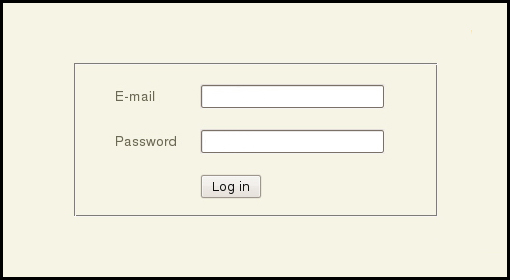
\includegraphics[scale=0.5]{images/login.jpg}\\
	\textbf{fig. 4.1.2.1} Form di login\\
\end{center}

La pagina di login, come si vede in figura 4.1.2.1, offre la possibiltà agli utenti come la segreteria didattica o i docenti di inserire il proprio username (corrispondente all'indirizzo email) e la relativa password per poter accedere alle funzioni private messe a loro disposizione.

In caso di login corretto verrà visualizzata nuovamente la pagina principale del prodotto SIGEOL, con in più i link a tutte le funzioni private accessibili.
In caso di errore nell'inserimento dell'indirizzo email o della password verrà visualizzato un messaggio di notifica di tale errore, come in figura 4.1.2.2.
Sarà immediatamente possibile reinserire i dati corretti e ritentare il login.

\begin{center}
	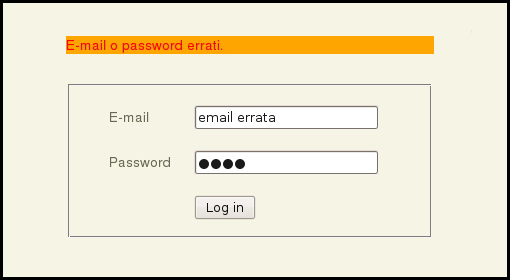
\includegraphics[scale=0.5]{images/login_errato.jpg}\\
	\textbf{fig. 4.1.2.2} Form dopo un login errato\\
\end{center}

Le funzioni accessibili alle due tipologie di utenti appena citate sono diametralmente opposte: nei successivi capitoli del presente documento verranno quindi solamente illustrate le funzioni dedicate alla segreteria didattica.
\subsection{Azioni richieste/permesse}
Ogni capitolo di questa sezione si riferisce ad una particolare funzione che il sistema SIGEOL mette a disposizione dell'utente segreteria didattica. Tali funzioni sono raggiungibili da un link presente nella pagina principale del sito dopo aver effettuato correttamente il login.
\subsubsection{Gestione Corsi di Laurea}
La pagina di gestione dei corsi di laurea mostra una lista di tutti i corsi inseriti dalla segreteria didattica.

E' possibile visualizzare le informazioni relative a quel corso di laurea cliccando sul nome del corso, ed è possibile eliminare quel particolare corso di laurea seguendo il link nominato `elimina`.
Per ogni corso di laurea sono elencati tutti curriculum che ne fanno parte: anche questi ultimi hanno le medesime funzioni di visualizzazione e eliminazione come appena illustrato per i corsi di laurea.

Per ogni curriculum, seguendo il link `Gestisci Insegnamenti`, è a disposizione una pagina in cui sono elencati tutti gli insegnamenti assegnati a quel particolare curriculum. E' data la possibilità di rimuovere o aggiungere uno o più insegnamenti: tale funzione è particolarmente utile per corsi di laurea che prevedono curriculum multipli, in quanto due o più curriculum all'interno dello stesso corso di laurea potrebbero condividere un particolare insegnamento.

Da notare che il rimuovere un insegnamento da un dato curriculum non equivale alla rimozione totale dell'insegnamento: per cancellare completamente un insegnamento non più necessario si prega di consultare la sezione `Gestione Insegnamenti` del presente documento.

Per ogni corso di laurea precedentemente inserito nel sistema SIGEOL è possibile impostare una scadenza entro cui i docenti devono terminare le loro operazioni di inserimento vincoli e preferenze: tale data è impostabile seguendo il link `Imposta data di termine inserimento vincoli`, disponibile a fianco di ogni singolo corso di laurea.

Sono poi disponibili, sia per i corsi di laurea sia per i curriculum, le funzionalità di inserimento e modifica, descritte più nel dettaglio qui di seguito:
\newline \newline
\begin{large}\textbf{Inserimento di un nuovo corso di laurea:}\end{large}

\begin{center}
	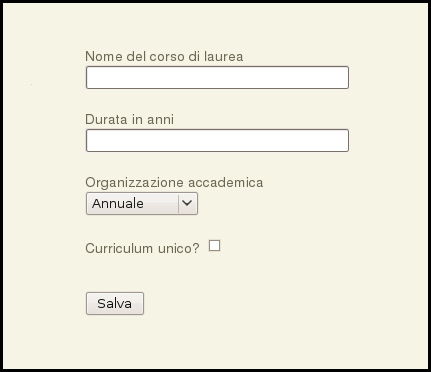
\includegraphics[scale=0.5]{images/nuovo_corso.jpg}\\
	\textbf{fig. 4.2.1.1} Form di inserimento di un corso di laurea\\
\end{center}

La pagina di inserimento di un nuovo corso di laurea, come visualizzato in figura 4.2.1.1, richiede:
\begin{itemize}
 \item inserimento del nome del corso di laurea: il nome non deve essere vuoto e deve contenere solamente caratteri o spazi. Sono vietati numeri o simboli. La lunghezza massima è fissata in 50 caratteri, compresi gli spazi.
 \item inserimento della durata in anni: deve essere inserito un numero compreso tra 1 e 6.
 \item scelta dell'organizzazione accademica: la scelta deve essere fatta tramite menu a tendina tra le varie opzioni proposte, che al momento sono annuale, semestri, trimenstri, quadrimestri. Serve a determinare in quanti periodi è suddiviso l'anno di quel determinato corso di laurea.
 \item nel caso il corso di laurea che si sta inserendo preveda un solo curriculum, è necessario selezionare la casella `Curriculum Unico` per crearlo automaticamente. Nel caso il corso di laurea preveda più curriculum, è sufficiente non selezionare tale opzione e inserire i vari curriculum successivamente. La scelta non è vincolante: è possibile eliminare o aggiungere curriculum a piacimento successivamente alla creazione del corso di laurea.
\end{itemize}
Al termine dell'inserimento dei dati richiesti, sarà sufficiente premere il bottone `Salva` per salvare il nuovo corso di laurea. Verrà di seguito visualizzata nuovamente la pagina principale di gestione dei corsi di laurea. 
\newline \newline
\begin{large}\textbf{Modifica dei dati di un corso di laurea:}\end{large}

\begin{center}
	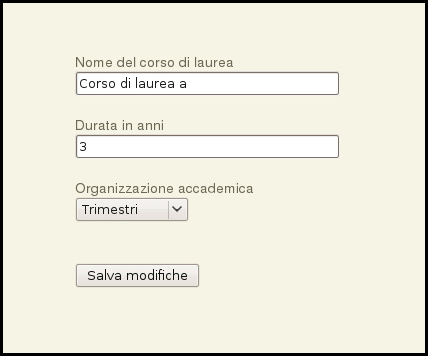
\includegraphics[scale=0.5]{images/modifica_corso.jpg}\\
	\textbf{fig. 4.2.1.2} Form di modifica di un corso di laurea\\
\end{center}

La modifica dei dati di un corso di laurea inserito precedentemente funziona similarmente alla inserimento appena illustrato, come visibile in figura 4.2.1.2. I campi che è possibile modificare sono:
\begin{itemize}
 \item nome
 \item durata in anni
 \item organizzazione accademica
\end{itemize}
Le regole da seguire per la loro compilazione sono identiche a quelle sopra illustrate per l'inserimento di un nuovo corso di laurea.
\newline \newline
\begin{large}\textbf{Inserimento di un nuovo curriculum:}\end{large}

\begin{center}
	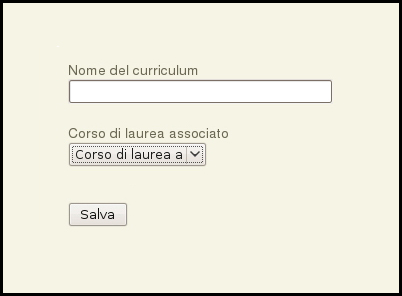
\includegraphics[scale=0.5]{images/nuovo_curriculum.jpg}\\
	\textbf{fig. 4.2.1.3} Form di inserimento di un curriculum\\
\end{center}

La pagina di inserimento di un nuovo curriculum, come visualizato in figura 4.2.1.3, richiede i seguenti campi:
\begin{itemize}
 \item inserimento del nome del curriculum: deve contenere solo caratteri o spazi e la sua lunghezza massima è fissata in 50 caratteri
 \item scelta del corso di laurea di cui il curriculum fa parte, tramite menu a tendina
\end{itemize}
Premendo il bottone `Salva` verrà salvato il curriculum e si verrà reindirizzati alla pagina di gestione dei corsi di laurea. Il nuovo curriculum appena creato sarà presente nella lista del relativo corso di laurea.
\newline \newline
\begin{large}\textbf{Modifica dei dati di un curriculum:}\end{large}

\begin{center}
	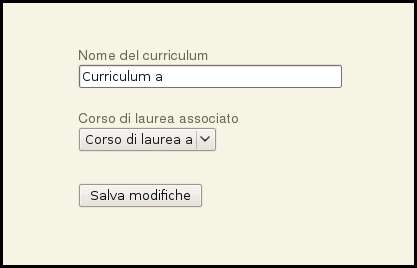
\includegraphics[scale=0.5]{images/modifica_curriculum.jpg}\\
	\textbf{fig. 4.2.1.4} Form di modifica di un curriculum\\
\end{center}

La pagina per modificare i dati di un curriculum esistente, visibile in figura 4.2.1.4, funziona in modo similare alla pagina di inserimento appena illustrata. I campi che è possibile modificare sono infatti:
\begin{itemize}
 \item nome del curriculum
 \item scelta del corso di laurea di cui il curriculum fa parte, tramite menu a tendina
\end{itemize}
Le regole da seguire per la loro compilazione sono identiche a quelle sopra illustrate per l'inserimento di un nuovo curriculum.
\subsubsection{Gestione Edifici}
La pagina di gestione degli edifici contiene una lista di tutti gli edifici a disposizione dalla segreteria didattica.

E' possibile consultare le informazioni relative ad un determinato edificio cliccando sul suo nome, oppure è possibile cancellare un determinato edificio dal sistema SIGEOL semplicemente seguendo il link `Elimina`.

E' importante ricordarsi di creare gli edifici necessari prima di creare una o più aule che sono presenti all'interno di quella struttura. In caso contrario, la nuova aula creata non potrà essere assegnata al corretto edificio.

Le funzioni di inserimento di un nuovo edificio e di modifica dei dati di un edificio già presente sono illustrate più in dettaglio qui di seguito:
\newline \newline
\begin{large}\textbf{Inserimento di un nuovo edificio:}\end{large}

\begin{center}
	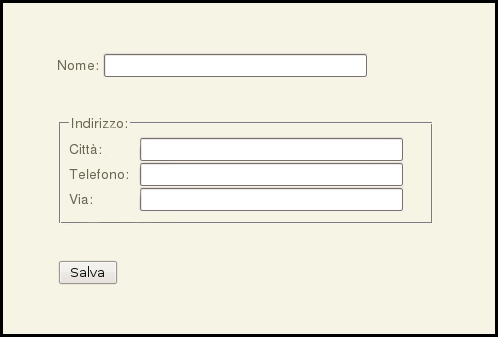
\includegraphics[scale=0.5]{images/nuovo_edificio.jpg}\\
	\textbf{fig. 4.2.2.1} Form di inserimento di un edificio\\
\end{center}

La pagina di inserimento di un nuovo edificio, come illustrato in figura 4.2.2.1, richiede l'inserimento obbligatorio dei seguenti dati:
\begin{itemize}
 \item nome dell'edificio: deve essere composto solamente da caratteri, numeri e spazi. La lunghezza massima del nome è stata fissata in 30 caratteri.
 \item città: il nome della città in cui si trova l'edificio deve essere composto solamente da caratteri o spazi. Anche in questo caso la lunghezza massima è fissata in 30 caratteri.
 \item numero di telefono: deve essere inserito nel formato `prefisso-numero`. Il prefisso può essere composto solamente da numeri e la sua lunghezza può variare da 2 a 4. Anche il numero segue le stesse regole, ma la lunghezza dev'essere compresa tra 6 e 8 cifre.
 \item via: si accettano caratteri, numeri e spazi. In questo caso la lunghezza massima è fissata in 50 caratteri, compresi gli spazi.
\end{itemize}
Al termine dell'inserimento di tutti i dati richiesti è sufficiente premere sul pulsante `Salva` per salvare l'edificio e il relativo indirizzo nel sistema SIGEOL.
Da questo momento è possibile inserire delle aule all'interno dell'edificio appena salvato.
\newline \newline
\begin{large}\textbf{Modifica dei dati di un edificio:}\end{large}

\begin{center}
	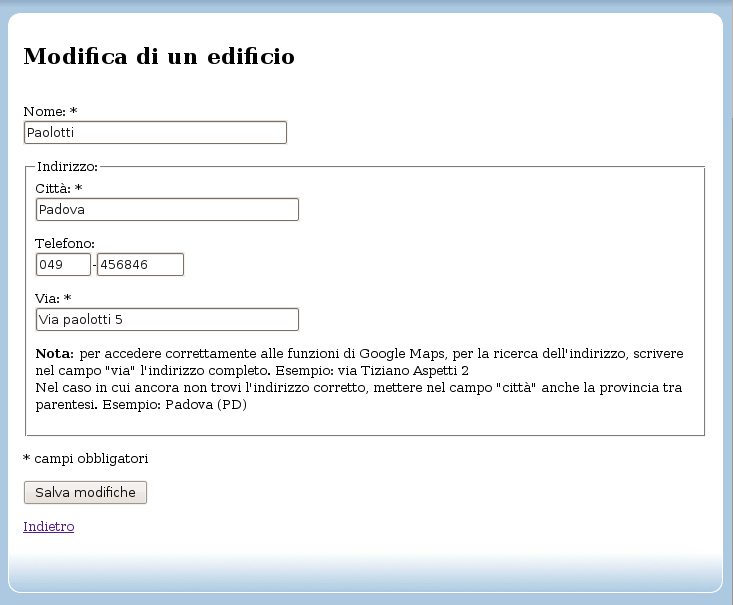
\includegraphics[scale=0.5]{images/modifica_edificio.jpg}\\
	\textbf{fig. 4.2.2.2} Form di modifica di un edificio\\
\end{center}

Come visualizzato in figura 4.2.2.2, la pagina di modifica dei dati di un edificio già presente nel sistema SIGEOL è di funzionamento simile alla pagina di inserimento appena descritta. Si possono modificare gli stessi dati inseriti in fase di creazione dell'edificio e le regole da rispettare per la modifica delle varie informazioni sono le stesse sopra elencate.

Al termine delle modifiche è sufficiente premere il bottone `Salva modifiche` per salvare le modifiche nel sistema SIGEOL.
\subsubsection{Gestione Aule}
La pagina di gestione delle aule contiene, in modo simile a tutte le altre pagine di amministrazione disponibili per la segreteria didattica, una lista delle aule a diposizione.
E' possibile consultare le informazioni relative ad una data aula cliccando sul link presente sul suo nome: all'interno di tale pagina è anche presente, tra gli altri dati, una lista dei corsi di laurea per cui quest'aula è messa a disposizione. La scelta di quest'ultimo particolare sarà illustrata nelle sezioni dedicate all'inserimento di una nuova aula e alla sua modifica.

E' anche data la possibilità di eliminare in modo permanente un aula dal sistema SIGEOL semplicemente seguendo il link `Elimina` presente a fianco di ogni aula.

I vincoli temporali di indisponibilità di ogni aula si possono inserire, gestire e cancellare seguendo il link `Gestione Vincoli`, disponibile a fianco di ogni singola aula. Tale pagina di gestione permette di inserire un nuovo vincolo di indisponibilità dell'aula tramite comodi menu a tendina, permette di cancellare vincoli già inseriti in passato e da la possibilità di modificare vincoli già presenti.

Le funzionalità di inserimento di una nuova aula e di modifica dei dati di una già presente sono illustrate in maggior dettaglio qui di seguito:
\newline \newline
\begin{large}\textbf{Inserimento di una nuova aula:}\end{large}

\begin{center}
	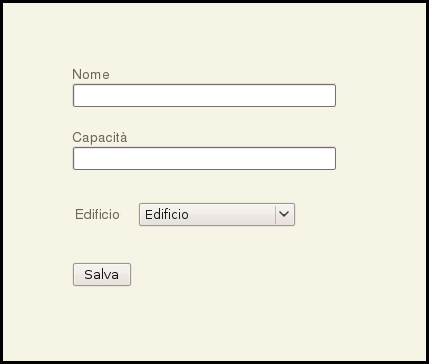
\includegraphics[scale=0.5]{images/nuova_aula.jpg}\\
	\textbf{fig. 4.2.3.1} Form di inserimento di un'aula\\
\end{center}

La pagina di inserimento di una nuova aula, come visualizzato in figura 4.2.3.1, richiede i seguenti dati:
\begin{itemize}
 \item nome dell'aula: deve essere non vuoto, può solamente contenere caratteri, numeri o spazi; la lunghezza massima è fissata in 30 caratteri. 
 \item capacità dell'aula: deve essere un numero intero compreso tra 1 e 1000
 \item scelta dell'edificio in cui l'aula è ubicata, tramite menu a tendina. Nel caso l'edificio non fosse ancora presente nel sistema SIGEOL, è necessario, prima della fase di creazione dell'aula, inserire i dati dell'edificio: per maggiori informazioni si prega di consultare la sezione `Inserimento di un nuovo edificio`.
\end{itemize}
Una volta inseriti correttamente tutti i dati è sufficiente premere il pulsante `Salva` per salvare la nuova aula.

Da notare che l'aula viene messa a disposizione automaticamente di tutti i corsi di laurea presenti nel sistema SIGEOL: se tale scelta non fosse corretta, sarà necessario passare alla fase di modifica dei dati dell'aula.
\newline \newline
\begin{large}\textbf{Modifica dei dati di un aula:}\end{large}

\begin{center}
	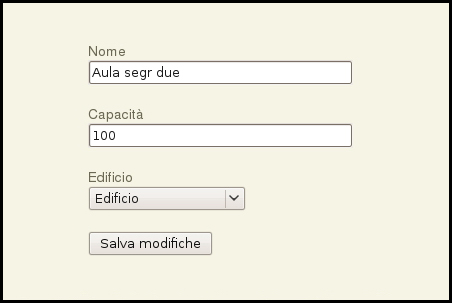
\includegraphics[scale=0.5]{images/modifica_aula.jpg}\\
	\textbf{fig. 4.2.3.2} Form di modifica di un aula\\
\end{center}

Come visualizzato in figura 4.2.3.2, la pagina di modifica dei dati di un aula già presente all'interno del sistema SIGEOL permette di aggiornare i seguenti dati:
\begin{itemize}
 \item nome dell'aula
 \item capacità dell'aula
 \item edificio in cui l'aula è ubicata, tramite menu a tendina
\end{itemize}
Le regole da rispettare per l'inserimento di questi dati sono le stesse sopra illustrate per la fase di inserimento di una nuova aula.
Premendo il bottone `Salva modifiche` i nuovi dati aggiornati saranno salvati nel sistema.

\begin{center}
	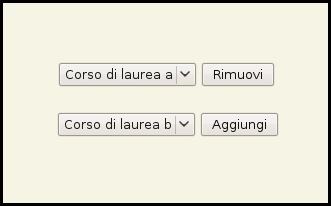
\includegraphics[scale=0.5]{images/modifica_aula_corso.jpg}\\
	\textbf{fig. 4.2.3.3} Form di aggiunta e rimozione delle disponibilità\\
\end{center}

Oltre ai campi per l'aggiornamento di questi dati, la pagina di modifica dei dati di un aula contiene una lista dei corsi di laurea per i quali quest'aula è messa a disposizione: sarà possibile modificare questa lista semplicemente usando i pulsanti `Aggiungi`, `Rimuovi` e i relativi menu a tendina, come illustrato in figura 4.2.3.3.

Nel caso vengano rimosse tutte le disponibilità, l'aula non è a disposizione di nessun corso di laurea, e pertanto non verrà mai considerata nella generazione degli orari di lezione.
E' pur sempre possibile rendere nuovamente disponibile quest'aula per qualche corso di laurea in seguito.
\subsubsection{Gestione Insegnamenti}
La pagina di gestione degli insegnamenti mostra un elenco degli insegnamenti presenti all'interno del sistema SIGEOL, raggruppati per corso di laurea.

Come per ogni altra pagina dedicata alla segreteria didattica, è possibile consultare le informazioni relative al corso di laurea o all'insegnamento prescelti semplicemente cliccando sul loro nome.
E' altresi possibile cancellare definitivamente un insegnamento dal sistema SIGEOL seguendo il link `Elimina` presente a fianco di ogni insegnamento.

Se un insegnamento presente in lista ha già un docente assegnato, sarà visualizzato il nome di tale docente.
In caso contrario sarà disponibile un link denominato `Assegna Docente`: seguendo questo link sarà possibile assegnare un dato docente all'insegnamento in questione. Da notare che il docente deve essere preventivamente invitato e registrato al sistema SIGEOL, altrimenti non sarà possibile assegnargli l'insegnamento.

Le funzioni di inserimento di un nuovo insegnamento e di modifica dei dati di uno già presente nel sistema saranno illustrate nel dettaglio qui di seguito:
\newline \newline
\begin{large}\textbf{Inserimento di un nuovo insegnamento:}\end{large}

\begin{center}
	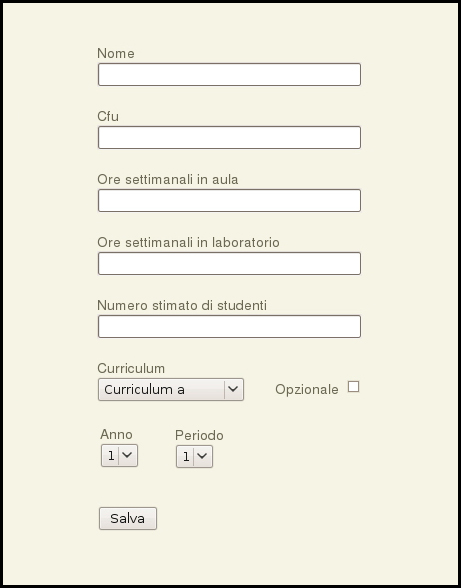
\includegraphics[scale=0.5]{images/nuovo_insegnamento.jpg}\\
	\textbf{fig. 4.2.4.1} Form di inserimento di un insegnamento\\
\end{center}

La pagina di inserimento di un nuovo insegnamento, come illustrato in figura 4.2.4.1, richiede obbligatoriamente i seguenti dati:
\begin{itemize}
 \item nome dell'insegnamento: deve essere composto solamente da caratteri, numeri o spazi; non può essere vuoto e la sua lunghezza massima è fissata in 30 caratteri.
 \item CFU: il numero dei crediti deve essere compreso tra 1 e 20
 \item ore di lezione settimanali in aula: deve essere un numero compreso tra 0 e 40
 \item ore di lezione settimanali in laboratorio: deve essere un numero compreso tra 0 e 40
 \item numero stimato di studenti: deve essere inserito un numero compreso tra 0 e 1000
 \item scelta del curriculum a cui l'insegnamento si riferisce, tramite menu a tendina
 \item opzionale: mettere la spunta nel caso il corso sia opzionale per il curriculum appena selezionato
 \item scelta dell'anno in cui il corso verrà tenuto nel curriculum selezionato, tramite menu a tendina
 \item periodo in cui il corso verrà tenuto: la scelta verrà fatta tramite menu a tendina e dovrà tener conto dell'organizzazione accademica del corso di laurea su cui si sta agendo.
\end{itemize}
Una volta inseriti tutti i dati, l'insegnamento verrà salvato nel sistema SIGEOL premendo il pulsante `Salva`.
\newline \newline
\begin{large}\textbf{Modifica dei dati di un insegnamento:}\end{large}
La pagina di modifica di un insegnamento già presente all'interno del sistema SIGEOL permette di aggiornare tutti i dati, mantenendo l'aspetto e i campi dato della pagina di inserimento di un nuovo insegnamento.
\subsubsection{Gestione Docenti}
La pagina di gestione dei docenti offre innanzitutto una lista dei docenti che sono stati invitati al sistema SIGEOL ma non hanno ancora completato la registrazione: questi docenti potranno essere gestiti e assegnati ai vari insegnamenti appena completeranno la loro registrazione.

A seguire è presente una lista dei docenti già correttamente registrati all'interno del sistema, raggruppata per corsi di laurea.
E' data la possibilità di:
\begin{itemize}
 \item eliminare completamente il docente dal sistema SIGEOL, seguendo il link `Elimina` presente a fianco di ogni docente
 \item aggiungere il docente prescelto ad un altro corso di laurea
 \item aggiungere dei privilegi al docente selezionato: questa funzione è particolarmente utile se si rivelasse la necessità di avere un docente che affianchi la segreteria didattica nella parte amministrativa del sistema SIGEOL (di default, il presidente del CCS è già un docente con tali privilegi, ma potrebbe nascere la necessità di avere un altro docente con qualche privilegio amministrativo).
\end{itemize}
E' anche disponibile, seguendo il link `Invito Docenti`, la seguente funzionalità:
\newline \newline
\begin{large}\textbf{Invito di un docente:}\end{large}

\begin{center}
	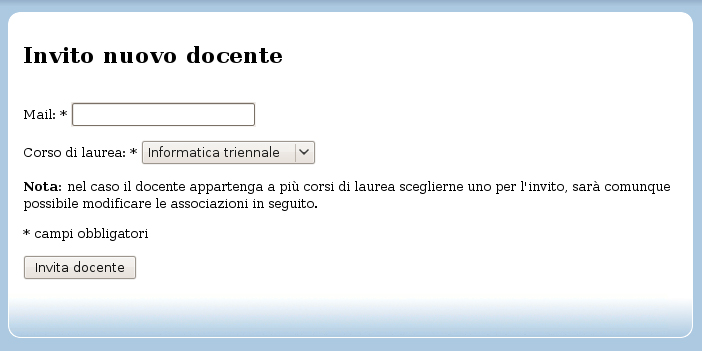
\includegraphics[scale=0.5]{images/invito_docenti.jpg}\\
	\textbf{fig. 4.2.5.1} Form di invito di un docente\\
\end{center}

Nella pagina di invito di un nuovo docente, come illustrato in figura 4.2.5.1, è sufficiente inserire l'indirizzo email a cui recapitare l'invito e, tramite menu a tendina, il corso di laurea per il quale il docente è richiesto.

Premendo il pulsante `Invita Docente` verrà automaticamente spedita un e-mail all'indirizzo specificato: tale e-mail conterrà delle brevi istruzioni che il docente dovrà seguire per completare la propria iscrizione al sistema SIGEOL.
Per ulteriori informazioni sulla procedura di attivazione dell'account di un docente si prega di consultare il documento \textsc{Manuale Utente Docente}.
\subsubsection{Cambio Password}
La pagina di cambio password permette semplicemente di modificare la password dell'account della segreteria didattica.

La procedura è particolarmente semplice: è sufficiente inserire la nuova password e premere il pulsante `Cambio Password`, come illustrato in figura 4.2.6.1.

\begin{center}
	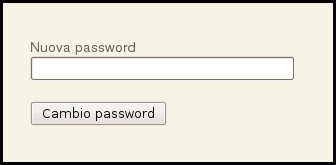
\includegraphics[scale=0.5]{images/cambio_password.jpg}\\
	\textbf{fig. 4.2.6.1} Form di cambio password\\
\end{center}


\subsubsection{Generazione dell'orario}
La pagina di generazione dell'orario di lezione permette alla segreteria didattica di far calcolare al sistema SIGEOL la miglior soluzione possibile di orario tenendo conto di tutti i dati che sono stati inseriti nelle precedenti fasi.

Al momento della generazione dell'orario, è data la possibilità di scegliere:
\begin{itemize}
 \item il corso di laurea di cui generare l'orario
 \item il periodo di cui calcolare l'orario, in base all'organizzazione accademica del corso di laurea prescelto (trimestri, semestri, ecc...)
\end{itemize}
Il calcolo dello schema d'orario non è istantaneo, ma potrà richiedere svariati minuti, in base anche alla complessità e al numero di dati inseriti.
La generazione dell'orario è indipendente dal sito internet del progetto: non è quindi necessario attendere la fine dei calcoli sulla pagina di generazione, ma è possibile compiere altre azioni o addirittura spegnere il calcolatore da cui è stata lanciata la richiesta.

Al termine del calcolo, l'orario sarà reso disponibile nella pagina principale del progetto SIGEOL.

Si ricorda che allo scadere della data limite di inserimento dei vincoli dei docenti (vedi sezione `Gestione corsi di laurea`) verrà automaticamente generato un orario di lezione per tutti i corsi di laurea, senza alcuna richiesta da parte della segreteria didattica. Potrà comunque essere generato nuovamente l'orario delle lezioni in seguito, per esempio dopo l'inserimento di nuove aule o di nuovi vincoli.
\subsection{Errori probabili e cause possibili}
L'inserimento dei dati nelle varie form da parte della segreteria didattica è seguito passo passo dal sistema SIGEOL: ogni dato è controllato e validato prima di essere salvato in modo persistente.

E' pertanto difficile, se non impossibile, inserire dati errati senza che questo venga segnalato.
La segnalazione degli errori avverrà in seguito alla pressione del pulsante di invio dei dati: verrà quindi visualizzata nuovamente la form da cui si era partiti, con in più la segnalazione dell'errore. Sarà quindi sufficiente correggere il dato che ha generato l'errore e premere nuovamente il pulsante di invio dei dati (che potrà essere `Salva`, `Salva Modifiche` o altro, in base alla form su cui si sta lavorando).

Per non andare incontro a segnalazioni continue di errori è necessario seguire le linee guida indicate nella sezione `Azioni richieste - permesse` del presente documento, di volta in volta consultando la sottosezione relativa alla funzionalità che si sta usando.

Si è deciso di non elencare tutti i possibili messaggi d'errore, in quanto tali messaggi sono talmente chiari e autoesplicativi da non necessitare di ulteriori definizioni.
\newpage
\section{Appendice}
\subsection{Glossario}




\modifiche
\end{document}
